Como se ha podido apreciar, existen multitud de aplicaciones relacionadas directa
o indirectamente con el \ac{OBD}--II, en parte por la longevidad del conector
en el mercado.

Sin embargo, todas o la gran mayoría de aplicaciones están destinadas a los profesionales
del sector, e incluso se ha aprovechado este conector para dificultar el acceso a
los datos del vehículo, habiendo de ir a un taller oficial para que puedan hacer
las reparaciones pertinentes.

Por otra parte, el parque de vehículos español es cada año más viejo debido a
diversos factores que no se van a analizar en este trabajo. Esto implica que cada
año más y más vehículos pierden el soporte por parte del fabricante y se vuelven
cada vez más costosos y complejos de mantener.

Para los no eruditos, el mundo del automóvil es el gran desconocido en donde una
serie de personas cualificadas se encargan del mantenimiento y correcto funcionamiento
del mecanismo que nos transporta por el mundo. Si bien es cierto que es necesaria
esta figura, hay una serie de buenas prácticas y actuaciones que pueden prevenir
tener que ir al mecánico de forma recurrente. Solo hace falta acceso a la información
de manera accesible.

Es por esto que nace \ac{VIMS}, un proyecto que pretende desarrollar un sistema completo
que consta de varias partes: un dispositivo embebido, un servidor y el usuario en sí
(figura \ref{fig:general-scheme}):

\begin{figure}[H]
  \centering
  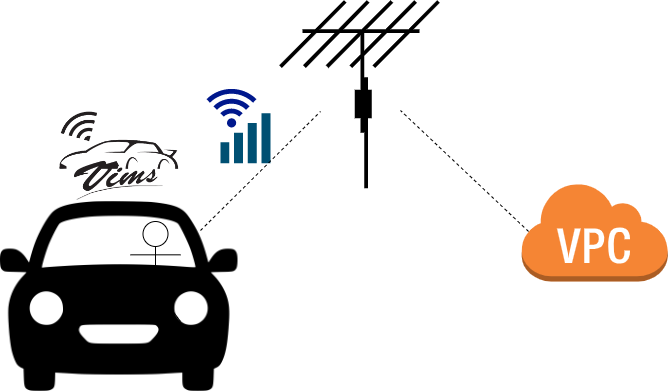
\includegraphics[width=\linewidth]{images/general-scheme.png}
  \caption{Esquema general que modela el modo de funcionamiento del sistema.}
  \label{fig:general-scheme}
\end{figure}

La idea fundamental detrás de este proyecto es la de devolverle a los usuarios
el control sobre su vehículo, ser conscientes de cómo funciona o, al menos, entender
mejor qué pueden hacer para mejorar tanto su estilo de conducción como la seguridad
al volante. De esta forma, con el dispositivo se espera también prevenir riesgos
ya que los propietarios y usuarios de los vehículos estarán informados en todo
momento de qué error pueda tener.

Como se prevé que este dispositivo sea utilizado por una gran variedad de usuarios
es crucial que sea accesible en términos de sencillez de manejo, entendimiento y
uso: evitar datos excesivamente técnicos, presentar la información más relevante
primero, etc.

Para ello, se hará uso de plataformas en la nube para gestionar, almacenar y presentar
la información al usuario y se contará con una aplicación móvil que permita un
fácil acceso a los datos del vehículo, tanto históricos como generados en el momento.

Al igual que otros trabajos previamente realizados, el proyecto se realiza sobre
las filosofías del código libre y del \textit{hardware} libre, que se traduce en
que todos los recursos (tanto físicos como \textit{software}) estarán disponibles
enteramente para cualquier persona interesada en ver cómo funciona, replicar el
proyecto por su cuenta y contar con plena potestad para mejorarlo, redistribuirlo
y trabajar con él (siempre bajo un prisma de reconocimiento al autor original
del trabajo regido por \textit{copyright}). Para ello, se ha decidido hacer uso
de la licencia MIT\footnote{Se pueden obtener más detalles sobre la licencia MIT
en la siguiente URL: \url{https://choosealicense.com/licenses/mit/}}.
